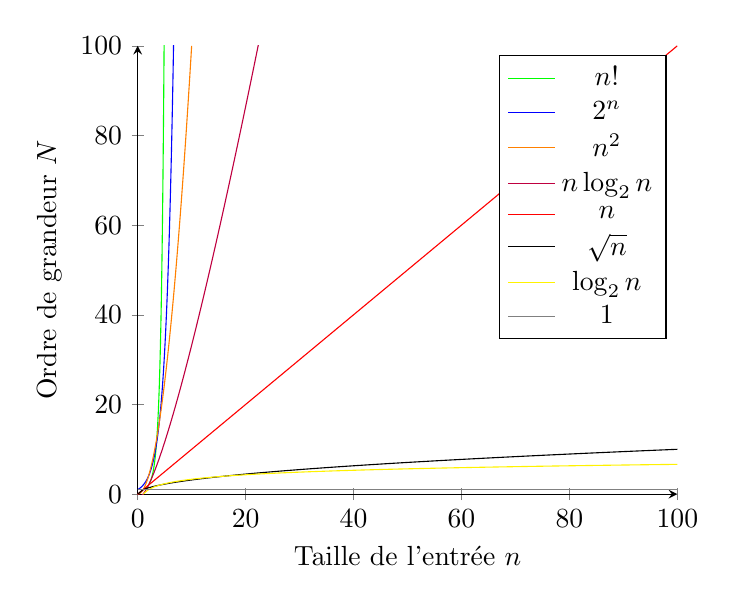
\begin{tikzpicture}[domain=0:4]
    \begin{axis}[
    axis lines = left,
    xlabel = {Taille de l'entrée \(n\)},
    ylabel = {Ordre de grandeur \(N\)},
    xmin=0, xmax=100,
    ymin=0, ymax=100,
    xtick={0,20,40,60,80,100},
    ytick={0,20,40,60,80,100}
    ]
    % plot y = x!
    \addplot [
        domain=1:7,
        samples=100,
        color=green,
    ]
    {sqrt(2*pi)*(x+1)^((x+1)-0.5)*exp(-(x+1))*exp(1/(12*(x+1)))};
    \addlegendentry{\(n!\)}
    % plot y = 2^x
    \addplot [
        domain=0:10,
        samples=100,
        color=blue,
    ]
    {2^x};
    \addlegendentry{\(2^n\)}
    % plot y = x^2
    \addplot [
        domain=0:10,
        samples=100,
        color=orange,
    ]
    {x^2};
    \addlegendentry{\(n^2\)}
    % plot y = x log_2 x
    \addplot [
        domain=0:30,
        samples=100,
        color=purple,
    ]
    {x * log2(x)};
    \addlegendentry{\(n \log_2 n\)}
    % plot y = x
    \addplot [
        domain=0:100,
        samples=100,
        color=red,
    ]
    {x};
    \addlegendentry{\(n\)}
    % plot y = sqrt(x)
    \addplot [
        domain=0:100,
        samples=100,
        color=black,
    ]
    {sqrt(x)};
    \addlegendentry{\(\sqrt{n}\)}
    % plot y = log_2 x
    \addplot [
        domain=0:100,
        samples=100,
        color=yellow,
    ]
    {log2(x)};
    \addlegendentry{\(\log_2 n\)}
    % plot y = 1
    \addplot [
        domain=0:100,
        samples=100,
        color=gray,
    ]
    {1};
    \addlegendentry{\(1\)}

    \end{axis}
\end{tikzpicture}